\documentclass{standalone}
\usepackage{tikz}
\usepackage{ctex,siunitx,bm}
\setCJKmainfont{Noto Serif CJK SC}
\usepackage{tkz-euclide,ninecolors}
\usepackage{amsmath}
\usetikzlibrary{patterns, calc}
\usetikzlibrary {decorations.pathmorphing, decorations.pathreplacing, decorations.shapes}
\newcommand{\posthead}[2][gray]{
  \begin{scope}[#2]
    \fill[left color=#1,right color= #1,middle color=#1!20](0,0)ellipse(0.05 and 0.02);
    \fill[left color=#1,right color= #1,middle color=#1!20](0.05,0)rectangle(-0.05,0.07);
    \fill[left color=#1,right color= #1,middle color=#1!20](-0.06,0.07)arc(-180:0:0.06 and 0.02)--(0.06,0.15)--(0.05,0.16)--(-0.05,0.16)--(-0.06,0.15)--cycle;
    \fill[#1!50!gray](0,0.16)ellipse(0.05 and 0.02);
    \foreach \x in {75,45,15,-15,-45,-75}
    {
      \draw[very thin,#1!50!gray]({0.05*sin(\x)},{0.16-0.02*cos(\x)})--({0.06*sin(\x)},{0.15-0.02*cos(\x)})--++(0,-0.08);
    }
  \end{scope}
}
\begin{document}
\small
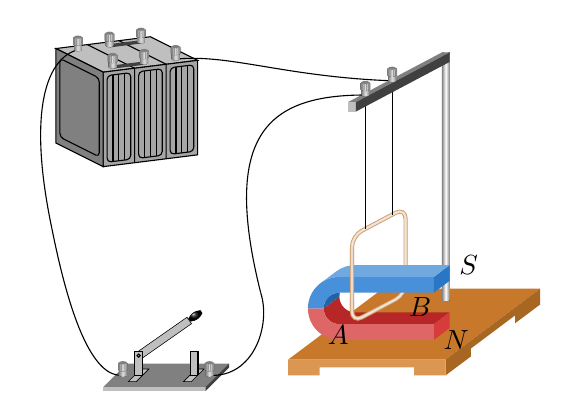
\begin{tikzpicture}[>=latex,yscale=1.0]
  \begin{scope}[xshift=-3cm,yshift=3cm]
    \draw[fill=lightgray](0,0)--(1.2,0.15)--(0.6,0.45)--(-0.6,0.3)--cycle;
    \draw[fill=gray!70](0,0)--(0,-1.2)--(1.2,-1.05)--(1.2,0.15)--cycle;
    \draw[fill=gray](0,0)--(0,-1.2)--(-0.6,-0.9)--(-0.6,0.3)--cycle;
    \draw(-0.2,0.35)--(0.4,0.05)--(0.4,-1.15)(0.2,0.4)--(0.8,0.1)--(0.8,-1.1);
    \draw[thin,rounded corners=0.5mm](-0.55,-0.825)--(-0.05,-1.075)--(-0.05,-0.075)--(-0.55,0.175)--cycle;
    \foreach \x/\y in {0/0,0.4/0.05,0.8/0.1}
    {
      \draw[thin,rounded corners=0.5mm](\x+0.05,\y-0.0437)--++(0.3,0.0375)--++(0,-1.10)--++(-0.3,-0.0375)--cycle;
      \draw[thin](\x+0.125,\y-0.0344)--++(0,-1.10);
      \draw[thin](\x+0.2,\y-0.025)--++(0,-1.10);
      \draw[thin](\x+0.275,\y-0.0156)--++(0,-1.10);
    }
    \draw(-0.320, 0.285)..controls(-0.750, 0.171)and(-0.952,-0.559)..(-0.651,-1.988);
    \draw(0.920, 0.165)..controls(1.590, 0.237)and(2.304,-0.059)..(3.670,-0.110);
    \draw[very thick,darkgray](0.52,0.115)--(0.12,0.065);
    \draw[very thick,darkgray](0.08,0.335)--(0.48,0.385);
    \posthead{xshift=1.2mm,yshift=0.65mm}
    \posthead{xshift=5.2mm,yshift=1.15mm}
    \posthead{xshift=9.2mm,yshift=1.65mm}
    \posthead{xshift=-3.2mm,yshift=2.85mm}
    \posthead{xshift=0.8mm,yshift=3.35mm}
    \posthead{xshift=4.8mm,yshift=3.85mm}
  \end{scope}
  \begin{scope}[yshift=5mm,xshift=1.2cm]
  \fill[brown6](-1.85,-1.15)--(0.15,-1.15)--(1.35,-0.25)--(-0.65,-0.25)--cycle;
  \fill[brown5]( 0.15,-1.35)--( 0.47,-1.11)--( 0.47,-1.01)--( 1.03,-0.59)--( 1.03,-0.69)--( 1.35,-0.45)--( 1.35,-0.25)--( 0.15,-1.15)--cycle;
  \fill[brown7]( 0.15,-1.15)--( 0.15,-1.35)--(-0.25,-1.35)--(-0.25,-1.25)--(-1.45,-1.25)--(-1.45,-1.35)--(-1.85,-1.35)--(-1.85,-1.15)--cycle;
  \end{scope}
  \fill[left color=gray, right color=gray,middle color=white](1.3,0.1)rectangle(1.4,3.25);
  \fill[red4](-0.2,0)arc(180:270:0.2)--++(1.2,0)--++(0.2,0.15)--++(-1.2,0)arc(270:180:0.2)--cycle;
  \fill[red5](1.2,-0.2)--++(0.2,0.15)--++(0,-0.2)--++(-0.2,-0.15)--cycle;
  \fill[red6](-0.4,0)arc(180:270:0.4)--++(1.2,0)node[right,text=black]{$N$}--++(0,0.2)--++(-1.2,0)arc(270:180:0.2)--cycle;
  \foreach \w in {80.60,40,20}
  {
    \draw[line width={1.5*sin(\w)},brown!\w,rounded corners](0.16,0.12)--(0.16,-0.18)--(0.84,0.18)--(0.84,1.28)--(0.5,1.1);
  }
  \fill[azure4](-0.2,0)arc(180:90:0.2)--++(0.2,0.15)arc(90:180:0.2)--cycle;
  \fill[azure6](-0.4,0)arc(180:90:0.4)--++(1.2,0)--++(0,-0.2)--++(-1.2,0)arc(90:180:0.2)--cycle;
  \fill[azure5](1.2,0.4)--++(0.2,0.15)node[right,text=black]{$S$}--++(0,-0.2)--++(-0.2,-0.15)--cycle;
  \fill[azure7](1.2,0.4)--++(0.2,0.15)--++(-1.2,0)arc(90:126.87:0.4)--++(-0.2,-0.15)arc(126.87:90:0.4)--cycle;
  \foreach \w in {80.60,40,20}
  {
    \draw[line width={1.5*sin(\w)},brown!\w,rounded corners](0.5,1.1)--(0.16,0.92)--(0.16,-0.18)--(0.5,0);
  }
  \draw(0.33,1.01)--++(0,1.7)(0.67,1.19)--++(0,1.7);
  \fill[gray](0.11,2.62)--(0.21,2.62)--(1.4,3.25)--(1.3,3.25)--cycle;
  \fill[lightgray](0.11,2.62)--(0.21,2.62)--(0.21,2.5)--(0.11,2.5)--cycle;
  \fill[darkgray](0.21,2.62)--(0.21,2.5)--(1.4,3.13)--(1.4,3.25)--cycle;
  \node at (0.16,-0.18) [below left,inner sep=1pt]{$A$};
  \node at (0.84,0.18) [below right,inner sep=1pt]{$B$};
  \draw( 0.330,2.710)..controls(-0.904,2.710)and(-1.506,2.218)..(-1.000,0.200);
  \posthead{xshift=0.33cm,yshift=2.71cm}
  \posthead{xshift=0.67cm,yshift=2.89cm}
  \begin{scope}[xshift=-3cm,yshift=-1cm]
    \fill[gray](0,0)--(1.3,0)--(1.6,0.3)--(0.3,0.3)--cycle;
    \fill[lightgray](0,0)--(1.3,0)--(1.3,-0.05)--(0,-0.05)--cycle;
    \fill[darkgray](1.3,0)--(1.3,-0.05)--(1.6,0.25)--(1.6,0.3)--cycle;
    \draw[fill=lightgray,very thin](0.32,0.07)--(0.42,0.07)--(0.58,0.23)--(0.48,0.23)--cycle(1.02,0.07)--(1.12,0.07)--(1.28,0.23)--(1.18,0.23)--cycle;
    \draw[fill=lightgray,very thin](0.45,0.4)--++(145:0.05)--++(35:0.8)--++(-55:0.1)--++(-145:0.8)--cycle;
    \draw[fill=lightgray,very thin](0.4,0.15)rectangle(0.5,0.45)(1.11,0.16)rectangle(1.21,0.46);
    \draw[fill=lightgray,very thin](1.1,0.15)rectangle(1.2,0.45);
    \draw(0.45,0.4)circle(0.02);
    \draw[very thin,ball color=black]([shift=(35:0.79)]0.45,0.4)--++(125:0.02)to[bend left]++(35:0.18)--++(-55:0.04)to[bend left]++(-145:0.18)--cycle;
    \draw(2.000,1.200)..controls(2.134,0.785)and(1.912,0.118)..(1.350,0.150);
    \draw(-0.651,2.012)..controls(-0.406,0.785)and(-0.109,0.118)..( 0.250,0.150);
    \posthead{xshift=0.25cm,yshift=0.15cm}
    \posthead{xshift=1.35cm,yshift=0.15cm}
  \end{scope}

\end{tikzpicture}
\end{document}